\documentclass[bibtex,nonblind]{template_artikel}
\totalwordcount{2314}
\title{Ulasan Artikel: Dilema Perpajakan Indonesia dalam Dua Perspektif Budiawan Sidik Arifianto}

\usepackage[hang]{footmisc}
\setlength{\footnotemargin}{0.5in}
\newcommand{\catatan}[1]{\footnote{\fontsize{10}{12}\selectfont\raggedright #1}}
\usepackage[hidelinks]{hyperref}
% The custom \author command takes THREE arguments:
% #1 = Author name
% #2 = Affiliation name
% #3 = Brief author profile, or anything that you'd usually put in a \thanks. Leave blank {} if there's nothing to be said.
\author{Farhan Aditya Ramadhan}
       {Universitas Indonesia}
       {Penyusun Laporan Teknis Berbasis LaTeX, Universitas Indonesia. (adin.ramaadin@gmail.com)}

%% These are used for the headers
\runningtitle{Proyek Latihan LaTeX – Analisis Kebijakan Ekonomi}
\runningauthor{Farhan Aditya Ramadhan} % 4 + Authors, Author On

%% Useful packages
\usepackage{amsmath}
\usepackage{graphicx}
\usepackage{rotating}

%% If you are using a custom figure or table environment from a package and it's not getting framed, add \makeframedenv{MyFigure} in the preamble, where the custom figure environment is \begin{MyFigure}...\end{MyFigure}.
%% Currently table, table*, figure, figure*, longtable, supertabular, sidewaystable and sidewaysfigure will be automatically framed.

%% Handy for setting wide tables/figures in landscape
\usepackage{pdflscape}
\usepackage{lipsum}
% Remove the current natbib/apacite setup and use this instead:
\usepackage[natbibapa]{apacite}
\bibliographystyle{apacite}
\renewcommand{\BAnd}{ dan }
\renewcommand{\AND}{ dan }

% Force proper APA formatting
\makeatletter
\renewcommand{\@biblabel}[1]{}  % Remove bibliography labels/keys
\makeatother

% Set hanging indent for references
\setlength{\bibhang}{0.5in}

\begin{document}
%%% DO NOT REMOVE THESE LINES. For automatic word count.
%TC:ignore
\begin{frontmatter}
\begin{abstract}
Pajak selalu menjadi kata yang sensitif di Indonesia. Wacana menaikkan tarif, bahkan hanya sekadar menyentuhnya, acapkali memicu kekhawatiran publik—terkadang logis, kadang juga emosional. Di tengah polemik kebijakan PPN 12 persen yang mencuat di akhir 2024, dua artikel Budiawan Sidik A. di Kompas.id berusaha menawarkan argumen: bahwa solusi tak semata-mata soal tarif, melainkan perbaikan tata kelola. Pesannya jelas—dan memang valid: sistem yang bocor tak bisa diatasi hanya dengan menaikkan angka. Akan tetapi, di balik rasionalitas itu, ada pertanyaan yang nyaris tak disentuh: dari mana biaya memperbaiki sistem itu berasal? Reformasi kelembagaan—mulai dari digitalisasi, birokrasi yang bersih, sampai investasi SDM—tak datang cuma-cuma. Ulasan ini ingin menggali lebih jauh paradoks tersebut: bahwa untuk memperbaiki tata kelola pajak, kita tetap perlu fiskal yang cukup—yang, ironisnya, mungkin hanya bisa dicapai lewat peningkatan penerimaan yang (lagi-lagi) sensitif secara politik. Di sinilah letak kegamangan kebijakan fiskal kita: antara ketakutan akan guncangan dan kebutuhan akan transformasi.
\end{abstract}
\end{frontmatter}

%%% DO NOT REMOVE THIS LINE. For automatic word count.
%TC:endignore

% Force consistent paragraph spacing
\setlength{\parskip}{0pt plus 1pt}
\setlength{\parindent}{1.5em}

% Include content from sections folder
\section{Pendahuluan}
\label{sec:Pendahuluan}
\setlength{\parskip}{0pt}
% Prevent footnote splitting dan flexible page layout
\interfootnotelinepenalty=10000
\clubpenalty=10000
\widowpenalty=10000
\raggedbottom

% APA 7 footnote command
\newcommand{\abaur}[1]{%
  \footnote{%
    \fontsize{10}{12}\selectfont%
    \setlength{\parindent}{0.5in}%
    \setlength{\parskip}{0pt}%
    \raggedright%
    #1%
  }%
}

\dropcap{Isu} pajak di Indonesia selalu sensitif. Setiap wacana kenaikan tarif—betapapun masuk akal dari sudut pandang ekonomi—acapkali disambut oleh pola yang sama: kekhawatiran publik, penolakan dari berbagai kalangan, dan akhirnya lahir kompromi politik. Episode PPN 12 persen pada akhir 2024 adalah contoh terbaru dari siklus ini. Dalam konteks tersebut, dua artikel Budiawan Sidik A. di \textit{Kompas.id}—“Kunci Pembangunan Ekonomi Bukan Hanya soal Besaran Pajak, melainkan Juga Tata Kelola” (24 Desember 2024) dan “Kebijakan Pajak yang Rasional Menstimulasi Kemajuan Ekonomi Nasional” (2 Januari 2025)—menawarkan perspektif yang relevan. Penempatan waktunya pun menarik: artikel pertama muncul di tengah gejolak opini publik, sedangkan artikel kedua hadir setelah pemerintah mengambil jalan tengah dengan membatasi PPN 12 persen hanya untuk barang mewah.

Sebagai peneliti di Litbang \textit{Kompas}, Budiawan menggunakan pendekatan berbasis data dan argumen yang tertata. Perbandingan lintas negara, analisis kelompok pendapatan, dan diagnosis struktural disusun dengan teliti (dan, dalam banyak hal, meyakinkan). Melalui tulisan-tulisannya, Ia tidak sekadar memperdebatkan soal tarif pajak dan justru mengajak kita melihat diskursus perpajakan dari sudut yang lebih luas dan, barangkali, lebih ``menenangkan'': bahwa masalah utama bukan hanya soal berapa persen tarif yang ditetapkan, melainkan seberapa efektif sistem pemungutannya bekerja. Lewat perbandingan lintas negara, termasuk negara-negara tetangga dan negara maju yang berhasil menaikkan rasio pajak mereka secara signifikan, Budiawan menyampaikan satu hal penting: Indonesia belum berada di posisi yang seharusnya.\catatan{Menariknya, beberapa negara dengan tarif PPN yang bahkan \textit{lebih rendah} justru mencatatkan \textit{tax to GDP ratio} yang jauh lebih tinggi. Artinya, masalah kita bukan pada tarif, tapi pada efektivitas dan kepatuhan—dan mungkin juga soal kepercayaan masyarakat terhadap sistem itu sendiri.} Tulisan-tulisannya, secara implisit, juga membawa semacam dorongan psikologis: bahwa \textit{we’re not doomed}—kita hanya belum optimal. Ketertinggalan ini bukan takdir; ia bisa diperbaiki, \texit{asalkan} kita mau mengubah cara pandang dan cara kelola. Dalam konteks rencana kenaikan tarif PPN menjadi 12 persen, Budiawan tidak serta-merta menolak, tetapi justru menawarkan penjelasan atas resistensi publik yang muncul. Di tengah kebutuhan belanja negara yang memang semakin besar, kekhawatiran masyarakat justru mengarah ke hal-hal yang lebih mendasar: potensi penurunan daya beli, perlambatan ekonomi, dan (ini penting) persepsi bahwa legitimasi sosial atas kebijakan fiskal belum benar-benar terbentuk.

Penelitian \textit{Kompas} yang dibawakan Budiawan, misalnya, menunjukkan bahwa penolakan terhadap kenaikan tarif datang dari hampir semua lapisan sosial—dari kelompok berpenghasilan tinggi hingga masyarakat berpendapatan rendah-dan mereka meminta penundaan pelaksanaan kebijakan hingga kondisi ekonomi membaik.\catatan{Model teoritis Timmons menunjukkan bahwa kepatuhan pajak bergantung pada persepsi warga tentang \textit{quid pro quo}—apa yang mereka terima sebagai imbalan dari pajak yang dibayar. Dalam konteks Indonesia, survei \textit{Kompas} yang dikutip Budiawan, menurut penulis ulasan ini, sebenarnya menyiratkan krisis legitimasi yang dalam: ketika semua lapisan sosial menolak kenaikan tarif, ini bukan sekadar soal ekonomi, tetapi soal kepercayaan. (Atau, dalam bahasa yang lebih kasar: ``Untuk apa saya bayar pajak kalau hasilnya tidak jelas?'')} Tanpa legitimasi yang kuat, kebijakan pajak yang baik di atas kertas pun bisa kehilangan daya dorongnya. Dan di titik ini, tulisan Budiawan tidak hanya menyodorkan kritik, tapi juga memberi harapan—bahwa ada jalan lain yang lebih masuk akal: bukan sekadar menaikkan tarif, tapi memperkuat kepercayaan, membangun sistem, dan memperbaiki hubungan antara negara dan warganya.

Kedua tulisan tersebut, menurut penulis, secara implisit juga berusaha menempatkan diskusi pajak dalam konteks struktural yang lebih luas—menyentuh aspek legitimasi sosial kebijakan fiskal, kapasitas negara dalam membangun kepercayaan publik, dan tantangan membiayai pembangunan tanpa menimbulkan beban berlebih pada masyarakat rentan. Namun, yang justru luput dibicarakan (dan inilah yang tulisan ini ingin gali lebih dalam) adalah kenyataan bahwa reformasi kelembagaan, betapapun esensialnya, tidak datang tanpa ongkos: modernisasi sistem informasi, perbaikan birokrasi (termasuk insentif agar aparatur tak tergoda rente), dan investasi jangka panjang dalam SDM semuanya membutuhkan biaya besar. Maka timbul pertanyaan yang tak mudah dielakkan: jika \textit{tax-to-GDP ratio} kita masih stagnan (dan di banyak kasus bahkan turun sejak pandemi), dari mana sumber daya fiskal untuk semua ini berasal—selain dari \textit{memaksa kenaikan} penerimaan pajak itu sendiri melalui kenaikan tarif umum PPN—yang secara administratif paling mudah dilakukan?\catatan{yang, ironisnya, justru menjadi titik tolak kegelisahan awal publik}. Di sinilah artikel Budiawan tampak konservatif: alih-alih mendorong terobosan fiskal yang ekspansif, ia seolah mengafirmasi \textit{status quo} dengan menekankan optimalisasi tata kelola (yang tentu penting, tapi apakah cukup?).

Dengan latar tersebut, ulasan ini akan dibagi ke dalam tiga bagian utama untuk memudahkan pembahasan. Bagian \textit{\hyperref[sec:Ringkasan]{Ringkasan Kedua Artikel}} akan memaparkan isi pokok kedua artikel Budiawan secara sistematis. Bagian \textit{\hyperref[sec:Analisis & Evaluasi]{Analisis}} akan menelusuri argumen, kerangka logis, serta asumsi yang melandasinya, termasuk implikasi yang mungkin luput dibahas. Terakhir, bagian \textit{\hyperref[sec:Kesimpulan]{Kesimpulan}} akan merangkum temuan utama ulasan ini serta memberikan refleksi terhadap relevansi dan keterbatasan argumen tersebut bagi diskursus perpajakan di Indonesia.
\clearpage

\section{Ringkasan Kedua Artikel}
\label{sec:Ringkasan}
\setlength{\parskip}{0pt}
% Prevent footnote splitting dan flexible page layout
\interfootnotelinepenalty=10000
\clubpenalty=10000
\widowpenalty=10000
\raggedbottom

Kedua artikel Budiawan Sidik A. menyajikan analisis komprehensif tentang perpajakan Indonesia melalui pendekatan data empiris dan perbandingan internasional. Bagian ini merangkum secara detail substansi, temuan, dan argumen yang dibangun dalam masing-masing artikel tanpa interpretasi atau evaluasi kritis.

\subsection{Artikel Pertama: Substansi dan Temuan Empiris}

Artikel \textit{``Kunci Pembangunan Ekonomi Bukan Hanya soal Besaran Pajak, melainkan Juga Tata Kelola''} dibuka dengan uraian ihwal hasil jajak pendapat \textit{Kompas} pada awal Desember 2024. Survei melibatkan 625 responden dari 38 provinsi dengan metode acak, memiliki \textit{margin of error} ±3,92 persen pada tingkat kepercayaan 95 persen.

\textbf{Temuan survei menunjukkan penolakan yang relatif seragam lintas lapisan sosial ekonomi:} kelompok ekonomi bawah menolak sebesar 50,6 persen, menengah bawah 29,1 persen, menengah atas 27,9 persen, dan atas 25,8 persen. Yang lebih penting, mayoritas dari semua lapisan itu menghendaki penundaan: 53 persen responden meminta kebijakan ditangguhkan hingga keadaan ekonomi membaik, sementara hanya 11,8 persen mendukung penerapan sesuai jadwal (dan ini menarik—karena jarang sekali ada “kebijakan fiskal” yang bisa menyatukan keresahan dari bawah sampai atas).

Budiawan kemudian menyinggung landasan yuridis, merujuk pada UU No. 7 Tahun 2021 tentang Harmonisasi Peraturan Perpajakan. Undang-undang tersebut menetapkan PPN 11 persen berlaku mulai 1 April 2022, serta PPN 12 persen selambatnya 1 Januari 2025. Pemerintah berpegang pada asas keadilan dan gotong royong: pihak yang mampu diharapkan berkontribusi sesuai undang-undang, sementara kelompok rentan dijanjikan perlindungan. Selain itu, khusus untuk barang kebutuhan pokok, pemerintah menyiapkan pembebasan pajak senilai Rp 265,6 triliun dan menanggung kenaikan 1 persen PPN untuk komoditas strategis seperti tepung terigu, gula industri, dan minyak goreng Minyakita. (ini bagian yang biasanya terdengar manis di podium—tetapi, seperti kita tahu, lapangan punya cara sendiri untuk ``menguji'' janji tersebut).

\textbf{Perbandingan internasional menjadi nadi argumentasi artikel ini.} Budiawan menyajikan data \textit{tax-to-GDP ratio} dan tarif PPN dari sembilan negara text{emerging market dan ASEAN}, sebagaimana tercantum dalam sebagaimana tercantum dalam \textit{Bagan~\ref{tab:international_comparison}}. Di sini Budiawan sedang membangun premis penting: tarif hanyalah wajah luar kebijakan, sedangkan efektivitas sistem terletak pada desain dan kapasitasnya—dan ini, kalau dibaca seksama, adalah kritik terhadap pendekatan \textit{business as usual} dalam fiskal Indonesia.

\begin{table}[hbt!]
\caption{Perbandingan Tarif PPN dan \textit{Tax-to-GDP Ratio} Negara-Negara \textit{Emerging Market} dan ASEAN}
\label{tab:international_comparison}
\centering
\begin{tabular}{lcc}
\textbf{Negara} & \textbf{Tarif PPN/VAT/GST (\%)} & \textbf{\textit{Tax-to-GDP Ratio} (\%)} \\
\midrule
Brasil & 17 & 24,67 \\
India & 18 & 17,33 \\
Turki & 20 & 16,4 \\
Thailand & 7 & 15,14 \\
Filipina & 12 & 14,62 \\
Vietnam & 10 & 12,8 \\
Singapura & 8 & 12,03 \\
Malaysia & 8 & 11,64 \\
\textbf{Indonesia} & \textbf{11} & \textbf{10,4} \\
\end{tabular}
\floatnote{Data tahun 2022 sebagaimana disajikan dalam artikel Budiawan. Indonesia ditampilkan dengan format tebal untuk menekankan posisinya sebagai objek analisis utama.}
\end{table}

Artikel juga menyoroti Penanaman Modal Asing (PMA) sebagai petunjuk perihal daya tarik investasi. Vietnam, misalnya, mencatat PMA 4 persen dari PDB; Singapura jauh lebih tinggi dengan 30 persen; sementara Indonesia hanya 1,61 persen (Dan di sini, Budiawan seakan menyelipkan sindiran halus: tarif pajak bukanlah pangkal tunggal persoalan—lihat saja, Vietnam tidak perlu menurunkan tarifnya serendah mungkin untuk mengundang arus modal). PMA yang tinggi berperan menciptakan lapangan kerja formal, memperluas basis pajak, dan pada akhirnya meningkatkan penerimaan negara. Budiawan menautkan fakta ini dengan mutu tata kelola perpajakan, yang pada gilirannya membentuk iklim usaha dan menentukan daya saing di percaturan global. Dengan kata lain, tarif hanyalah wajah luar kebijakan, sedangkan tata kelola adalah ruhnya—dan di sinilah pekerjaan rumah Indonesia tampak paling berat.

\textbf{Kesimpulan} artikel pertama menegaskan bahwa Vietnam dan Singapura patut dijadikan rujukan—bukan untuk meniru tarifnya semata, tetapi dalam pengelolaan pajak dan kemampuannya menghadirkan investasi asing. Budiawan menyiratkan tesis yang cukup gamblang: persoalan Indonesia bukan kekurangan instrumen fiskal, melainkan keterbatasan kapasitas dan tata kelola.

\subsection{Artikel Kedua: Analisis Pascakeputusan dan Perbandingan Regional}

Artikel \textit{``Kebijakan Pajak yang Rasional Menstimulasi Kemajuan Ekonomi Nasional''} dibuka dengan validasi terhadap langkah pemerintah membatasi PPN 12 persen hanya untuk barang mewah. Budiawan merujuk data BPS 2024 yang menunjukkan masyarakat golongan atas di Indonesia berjumlah 1{,}07 juta orang---sekitar 0{,}38 persen populasi---dengan pengeluaran di atas Rp 9{,}9 juta per bulan. Segmen ini kecil, tetapi strategis; pemerintah agaknya sadar bahwa legitimasi publik lebih mudah dijaga bila kebijakan diarahkan ke kelompok yang dinilai mampu menanggungnya.

\textbf{Analisis struktur pengeluaran menyingkap kontras pola konsumsi yang tajam.} Kelompok atas memiliki porsi pengeluaran untuk kebutuhan pokok (pangan, sandang, papan) yang jauh lebih kecil dibanding kelompok menengah-bawah, sementara belanja untuk hiburan, kendaraan, pendidikan, dan kesehatan---yang kerap masuk kategori mewah---jauh lebih besar. Sebaliknya, kelompok menengah menyumbang 81{,}49 persen dari total pengeluaran nasional pada 2024. Dengan kata lain, jika tujuan fiskal adalah memperluas basis penerimaan, maka penyesuaian kebijakan perlu menyentuh struktur pengeluaran riil masyarakat, bukan sekadar menyesuaikan tarif yang tampak efektif di atas kertas.

Artikel ini kemudian melebarkan cakrawala analisis ke tingkat regional, membandingkan data PDB, pertumbuhan ekonomi, pendapatan per kapita, dan tarif PPN di negara-negara ASEAN. Indonesia, dengan PDB USD 1.371{,}17 miliar, memang ekonomi terbesar ASEAN. Namun, dengan tarif PPN 11 persen dan \textit{tax ratio} 10{,}31 persen, posisinya justru berada di peringkat terbawah dalam efektivitas fiskal di kawasan. Paradoks ini kembali hadir: besar di ukuran, namun tertatih dalam pengelolaan; ibarat raksasa yang belum piawai mengatur langkahnya sendiri.

\textbf{Diagnosis masalah struktural dipaparkan dengan terang.} Budiawan menandai tiga simpul persoalan utama:
\begin{enumerate}
    \item Ketidakakuratan pendataan barang dan jasa di pasar domestik,
    \item Pelaporan data fiktif oleh pelaku usaha untuk mengurangi kewajiban pajak, 
    \item Praktik kolusi antara oknum perpajakan dengan wajib pajak ``nakal''.
\end{enumerate}
Ia menekankan perlunya penegakan hukum yang tegas dan pembenahan tata kelola perpajakan yang bersih. Isu ini terdengar akrab, nyaris menjadi refrein lama; namun pengulangannya memberi sinyal bahwa masalahnya bukan teknis belaka, melainkan struktural---tak cukup diselesaikan dengan tambalan kecil di permukaan.

Analisis Budiawan juga menelaah pendorong utama perekonomian ASEAN: konsumsi rumah tangga (50--70 persen PDB di mayoritas negara), investasi atau pembentukan modal tetap bruto (20--30 persen), dan belanja pemerintah (10--16 persen). Indonesia mencatat belanja pemerintah yang relatif rendah (7{,}45 persen), jauh di bawah Malaysia (11{,}95 persen), Thailand (16{,}64 persen), dan Singapura (10{,}23 persen). Rendahnya belanja ini, dibaca bersama \textit{tax ratio} yang kecil, menunjukkan bahwa negara belum memanfaatkan ruang fiskal untuk memacu pertumbuhan---padahal, ruang itu justru krusial untuk memperkuat basis penerimaan di masa depan.

\textbf{Data FDI \textit{inflows} dan \textit{outflows} menyingkap lanskap investasi regional.} Singapura memimpin dengan FDI \textit{inflow} 34{,}95 persen PDB dan \textit{outflow} 12{,}56 persen, menegaskan perannya sebagai \textit{hub} keuangan kawasan. Vietnam konsisten menarik FDI 4--5 persen PDB. Sementara itu, Indonesia stagnan di \textit{inflow} 1{,}61 persen dan \textit{outflow} minimal 0{,}52 persen. Angka-angka ini menegaskan posisi Indonesia: besar secara ekonomi, namun belum menjadi magnet investasi regional. Dan di era arus modal yang lincah, posisi ini bukan sekadar statistik, melainkan peringatan.

Artikel ini---sebagaimana artikel pertama---ditutup dengan rekomendasi yang menitikberatkan pada tiga kata kunci: transparansi, akuntabilitas, dan efektivitas penggunaan hasil pajak. Budiawan menegaskan, legitimasi sosial kebijakan fiskal hanya akan tegak bila masyarakat menyaksikan hasil konkret dari pajak yang dibayarkan. Dalam hal ini, Vietnam dan Singapura kembali dihadirkan sebagai rujukan---bukan semata pada level teknis, tetapi pada integrasi antara kebijakan fiskal, tata kelola, dan strategi pembangunan ekonomi. Seolah Budiawan ingin berbisik: kita tidak kekurangan instrumen; yang kita perlukan adalah kemauan dan kapasitas untuk memanfaatkannya dengan sungguh-sungguh.

\section{Analisis dan Evaluasi}
\label{sec:Analisis & Evaluasi}
\setlength{\parskip}{0pt}
% Prevent footnote splitting dan flexible page layout
\interfootnotelinepenalty=10000
\clubpenalty=10000
\widowpenalty=10000
\raggedbottom

Setelah memetakan substansi kedua artikel Budiawan secara rinci, tibalah saatnya menimbang secara kritis kekuatan dan kelemahan argumentasinya. Analisis ini ditempatkan dalam kerangka literatur \textit{fiscal capacity} yang lebih luas—terutama dengan mempertimbangkan paradoks sumber daya fiskal yang telah kita singgung di pendahuluan. Paradoks ini, sebagaimana yang akan kita lihat, bukan sekadar soal teknis; ia adalah simpul persoalan yang—anehnya—terus kembali dalam wacana fiskal Indonesia, seolah menjadi motif berulang dalam narasi kebijakan pajak kita.

\subsection{Kekuatan Artikel: Data yang Meyakinkan dan \textit{Political Timing} yang Tepat}

Kekuatan utama pendekatan Budiawan terletak pada ketajamannya membaca lanskap empiris dan celah retorika kebijakan. Survei \textit{Kompas} yang dikutipnya bukan hanya metodologis—625 responden, 38 provinsi, \textit{margin of error} ±3,92 persen—tetapi juga politis dalam efeknya. Hasil survei yang menunjukkan penolakan publik secara \textit{cross-cutting} memberi legitimasi pada klaim bahwa resistensi terhadap kenaikan tarif bukanlah ekspresi emosional yang temporer, melainkan refleksi dari kegelisahan yang lebih dalam dan sistemik.

Budiawan juga jeli memanfaatkan perbandingan internasional. Kondisi yang Ia tampilkan: Thailand dengan GST 7 persen memiliki tax ratio 15,14 persen, sementara Indonesia dengan PPN 11 persen hanya 10,4 persen. Di sini, Budiawan berhasil melakukan \textit{reframing}: alih-alih bertanya “perlukah tarif dinaikkan?”, ia menggeser fokus menjadi “mengapa sistem kita gagal memobilisasi penerimaan?”—suatu pergeseran yang subtil tetapi strategis.

\textit{Strategic positioning} kedua artikel juga menunjukkan kejelian politik yang patut dicatat. Artikel pertama hadir sebagai suara akademis yang kredibel di tengah riuhnya opini publik, sementara artikel kedua memberikan validasi empiris atas keputusan pemerintah tanpa terkesan oportunistik. \textit{(Timing}-nya terasa tepat: Budiawan berhasil menempatkan dirinya sebagai peneliti yang konsisten dengan analisis berbasis bukti di tengah polarisasi—posisi yang tidak mudah dipertahankan di lanskap kebijakan Indonesia.)

\subsection{Paradoks Fundamental: Masalah "Ayam dan Telur" yang Tak Kunjung Terurai}

Artikel tersebut tajam, tetapi dibaliknya, tersembunyi paradoks yang tak kunjung terurai (yang sudah disinggung pada bagian \hyperref[sec:Pendahuluan]{\textit{Pendahuluan}}). Budiawan menyarankan bahwa penguatan institusi adalah prasyarat untuk peningkatan kapasitas pajak. Akan tetapi, reformasi institusi itu sendiri memerlukan sumber daya—yang ironisnya, baru bisa diperoleh bila penerimaan fiskal (dalam hal ini pajak) telah membaik

Kedua artikel Budiawan, dengan cara yang hampir tidak disengaja, menghadirkan \textit{puzzle} yang akrab bagi siapa pun yang pernah bergulat dalam perdebatan fiskal Indonesia: bagaimana mungkin kita membenahi sistem perpajakan—yang, implikasinya, juga berarti memperkuat institusi negara dan membangun kapasitas negara (\textit{state capacity})—tanpa terlebih dahulu memiliki sumber daya untuk membiayai perbaikan itu sendiri? Sumber daya itu pada gilirannya diharapkan datang dari penguatan \textit{tax capacity}—yang, sebagaimana diingatkan Brautigam et al. (2008), adalah sumber penerimaan paling andal dan berkelanjutan bagi \textit{statebuilding}.  
\catatan{Paradoks ini mengingatkan pada apa yang oleh literatur ekonomi politik disebut \textit{bootstrapping problem}—membangun institusi pajak butuh dana, tetapi dana itu hanya tersedia jika institusi pajak sudah kuat. Sebuah sirkularitas yang membuat kebijakan terjebak dalam pusaran mandek: untuk menggerakkan A, perlu B; tapi B hanya tersedia jika A sudah berjalan.}  

Studi IMF (2023), yang hasilnya dipaparkan pada \hyperref[tab:tab:tax_potential_effort]{\textit{Bagan}~\ref{tab:tax_potential_effort}}, menunjukkan bahwa negara-negara LIDCs memiliki potensi pajak sekitar 19,9 persen PDB, tapi realisasinya hanya 12,1 persen. Indonesia bahkan lebih rendah dari itu. Maka persoalannya bukan hanya soal moral atau komitmen birokratik—tapi soal struktur: sistem kita tidak diberi cukup "amunisi" untuk bertempur. Reformasi kelembagaan, betapapun esensialnya, tidak datang tanpa ongkos. Modernisasi sistem informasi perpajakan menuntut investasi bernilai miliaran rupiah; perbaikan birokrasi—termasuk penyediaan insentif agar aparatur tak tergoda rente—memerlukan skema kompensasi yang kompetitif; dan investasi jangka panjang dalam sumber daya manusia hanya mungkin berlangsung dengan dukungan anggaran yang berkelanjutan \citep{chang_2011_institutions}.\catatan{Ironisnya, semua itu membutuhkan kapasitas fiskal yang justru belum kokoh—lingkaran yang sulit diputus.}  

\begin{table}[hbt!]
\caption{Potensi Pajak dan \textit{Tax Effort} Berdasarkan Kelompok Negara (2020)}
\label{tab:tax_potential_effort}
\centering
\begin{tabular}{1111}
\resizebox{\columnwidth}{!}{%
\begin{tabular}{@{}lll@{}}
\toprule
\multicolumn{1}{c}{\textbf{Kelompok Negara}} & \multicolumn{1}{c}{\textbf{Potensi Pajak (\%PDB)}} & \multicolumn{1}{c}{\textbf{Peneriman Aktual (\% PDB)}} \\ \midrule
Advanced Economies (AEs)                & 26,0 & 24,6 \\
Emerging Market Economies (EMEs)        & 22,5 & 16,6 \\
Low-Income Developing Countries (LIDCs) & 19,9 & 12,1 \\ \bottomrule
\end{tabular}%
}
\end{tabular}
\floatnote{\textit{Sumber:} IMF (2023). \textit{Tax effort} didefinisikan sebagai rasio antara penerimaan aktual dan potensi pajak. Nilai yang semakin mendekati 1,0 menunjukkan efektivitas mobilisasi pajak yang semakin tinggi.}
\end{table}   

\subsection{Konservatisme Fiskal yang Tidak Disadari}
Di tengah kenyataan bahwa \textit{tax-to-GDP ratio} Indonesia masih stagnan, bahkan di beberapa periode pascapandemi cenderung menurun, muncul pertanyaan yang sulit dielakkan: dari mana sumber daya fiskal untuk membiayai reformasi tersebut berasal? Pilihan yang secara administratif paling mudah—dan yang juga menjadi pangkal kegelisahan publik—adalah mendorong kenaikan penerimaan pajak melalui tarif umum PPN.

Evaluasi yang adil juga harus mengidentifikasi potensi bias dalam pendekatan Budiawan. Dengan menekankan optimalisasi sistem yang ada dan menghindari diskusi tentang \textit{substantive tax increases}, ia mungkin secara tidak sadar mengafirmasi \textit{status quo} dan menghindari reformasi fiskal yang lebih \textit{bold} tapi diperlukan.

Dalam konteks kebutuhan investasi besar—baik untuk infrastruktur, penanggulangan perubahan iklim, maupun pengembangan sumber daya manusia—pertanyaan mengenai kecukupan (\textit{adequacy}) dari ruang fiskal yang ada menjadi penting. Literatur menunjukkan bahwa banyak negara berkembang perlu memperluas \textit{fiscal space} secara signifikan untuk mencapai target pembangunan \citep{murshed_2020_fiscal}.

Pendekatan yang terlalu fokus pada \textit{efisiensi} dari sistem yang ada, tanpa mengalamatkan \textit{kecukupan} dari \textit{tingkat penerimaan yang dibutuhkan secara menyeluruh},  berpotensi tidak memadai untuk menjawab kebutuhan pembangunan Indonesia. \catatan{Ini adalah observasi, yang tidak unik, tentang mengenai konsekuensi tak terduga dari kerangka analisis} yanf sering orang pilih. Kadang-kadang, apa yang tampak sebagai pragmatisme \textit{incremental} justru dapat membatasi \textit{policy imagination} tentang apa yang mungkin dan perlu dilakukan. Di sinilah terlihat kehati-hatian Budiawan—atau, jika menggunakan istilah lain, konservatisme fiskal. Alih-alih mengadvokasi terobosan yang bersifat ekspansif, ia lebih memilih menekankan optimalisasi tata kelola. Penting, tentu saja, tetapi pertanyaannya: apakah itu cukup? Atau, meminjam peribahasa lama, bisakah kita mengubah wajah kebijakan hanya dengan merapikan cermin, tanpa menyentuh ruang di baliknya?

Sebelum menilai lebih jauh, perlu diakui bahwa langkah kenaikan tarif umum PPN yang sempat menuai resistensi publik sesungguhnya merupakan kebijakan yang, dari sisi penerimaan, cukup rasional. \textit{Tax-to-GDP ratio} Indonesia yang stagnan selama lebih dari satu dekade, dengan kebutuhan pembiayaan pembangunan yang kian mendesak, menuntut adanya sumber pendapatan yang relatif cepat, stabil, dan secara administratif dapat diandalkan. Kenaikan PPN tahun lalu—meski tidak populer—secara teknis adalah langkah yang sulit dihindari. Kontribusi PPN terhadap penerimaan negara cukup signifikan dan relatif tahan terhadap fluktuasi ekonomi \citep{saptono_2022_institutional,arvin_2021_are}. 

Pilihan menaikkan tarif umum PPN sering dianggap langkah yang paling mudah secara administratif—sebagaimana dicatat dalam literatur fiskal \citep{brautigam_2008_taxation, timmons_2005_the, akanbi_2019_state, addison_2018_fiscal, gaspar_2016_tax, iswahyudi_2021_getting}. Alasannya tidak hanya terletak pada kesederhanaan mekanisme: PPN memiliki basis pemungutan yang luas, tingkat kepatuhan yang relatif lebih baik dibanding pajak langsung, dan—ini penting dalam konteks Indonesia—lebih tahan terhadap tantangan informalitas. Dengan lebih dari separuh tenaga kerja masih berada di sektor informal (ILO, 2023) dan estimasi \textit{shadow economy} yang berkisar 19–30 persen PDB (IMF; ADB), basis pajak langsung menjadi sempit dan sulit diawasi. PPN, sebaliknya, dipungut di titik konsumsi formal yang relatif lebih mudah dilacak. Ibaratnya, ini jalur tol fiskal: tanpa perlu menembus hutan belantara informalitas, penerimaan negara tetap mengalir.  

Korelasi antara tingkat pajak dan kualitas institusi—sebagaimana terlihat pada \textit{Gambar}~\ref{fig:pajak_institusi}—terlihat konsisten. Namun, tentu penulis menyadari bahwa korelasi tidak otomatis berarti kausalitas. Peningkatan rasio pajak terhadap PDB, jika hanya dibaca dari grafik, belum tentu menjadi penyebab langsung menguatnya kapasitas institusi. \catatan{Dan di sini, godaan untuk tergesa-gesa menyimpulkan hubungan sebab-akibat memang selalu mengintai.}  

\begin{figure}[hbt!]
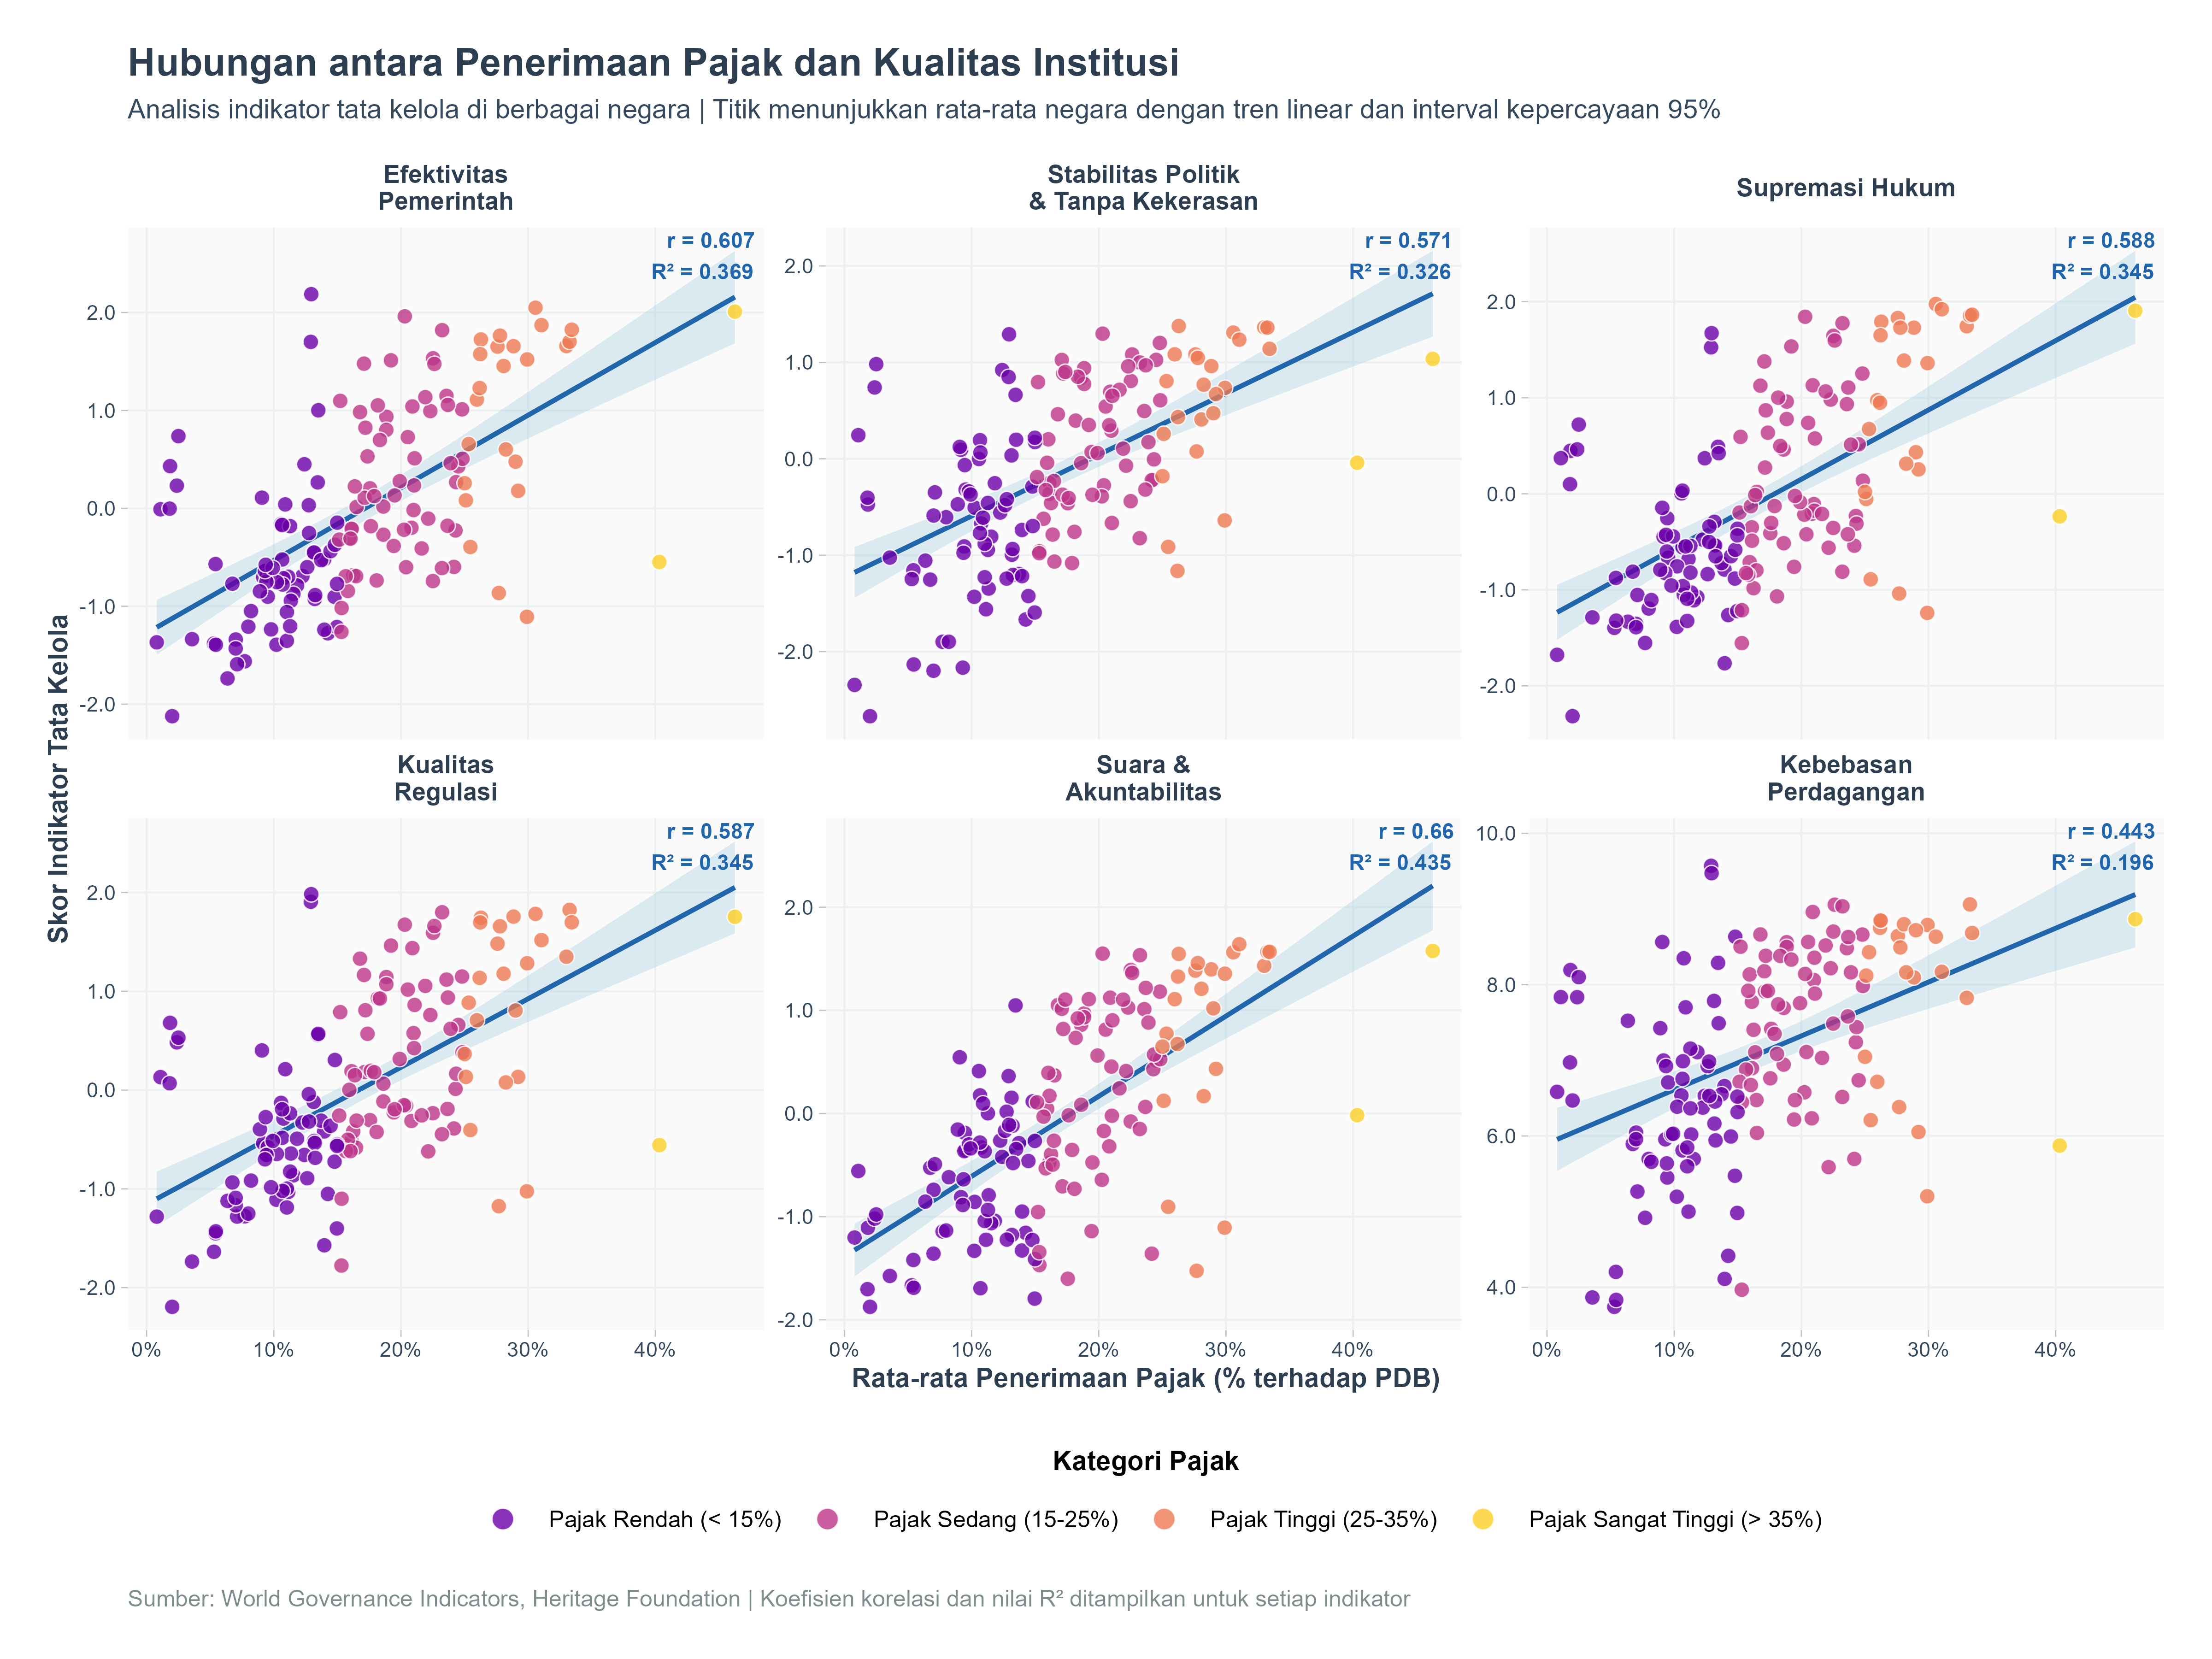
\includegraphics[width=\linewidth]{analisis_pajak_tata_kelola.png}
\caption{Hubungan Antara Tingkat Pajak dan Kualitas Institusi.}
\label{fig:pajak_institusi}

\floatnote{Visualisasi ini menunjukkan hubungan antara persentase penerimaan pajak terhadap PDB dan berbagai indikator tata kelola pemerintahan di negara-negara terpilih. Setiap panel menampilkan regresi linier dan rentang kepercayaan 95\%.
\newline
\textit{Sumber data:} ICTD/UNU-WIDER Government Revenue Dataset (2023); World Governance Indicators (2023); Heritage Foundation (2023). Visualisasi dibuat oleh Penulis menggunakan R.}
\end{figure}

Literatur memberi penjelasan yang lebih hati-hati. \citet{akanbi_2019_state}, melalui panel Granger causality test, menemukan hubungan kausalitas dua arah antara kapasitas pajak dan kualitas institusi. Menggunakan Panel Vector Error Correction Model, ia menunjukkan bahwa keduanya saling memperkuat di berbagai kelompok negara. Artinya, membangun kapasitas pajak dan institusi sebaiknya dilakukan beriringan—bukan menunggu yang satu selesai baru yang lain dimulai.  Arvin et al. (2021) sampai pada kesimpulan serupa, yaitu pertumbuhan ekonomi per kapita di negara-negara berpendapatan rendah dan menengah ke bawah dipengaruhi signifikan oleh penerimaan pajak, belanja pemerintah, dan kualitas institusi—terlepas dari jenis pajak yang digunakan.  Gaspar et al. (2016) menambahkan dimensi menarik: adanya ambang batas (\textit{tipping point}) rasio pajak terhadap PDB (bisa merujuk ke \textit{\hyperref[fig:view]{Gambar 2}}). Mereka menemukan bahwa ketika rasio tersebut mencapai sekitar 12,75 persen, PDB riil per kapita cenderung meningkat tajam dan berkelanjutan dalam dekade berikutnya. Rata-rata negara yang naik dari 12,5 persen menjadi 13 persen \textit{tax-to-GDP} berpeluang memiliki PDB per kapita sekitar 7,5 persen lebih besar dibanding negara sejenis yang tetap berada di bawah ambang tersebut. \textit{Seolah ada “pintu rahasia” yang baru terbuka begitu ambang ini terlampaui.}

Dari sini, ada satu implikasi yang tampaknya luput diperhitungkan Budiawan: konsep \textit{tax tipping point} ini mengindikasikan bahwa negara-negara dengan kapasitas pajak di bawah 12,75 persen dari PDB rawan terjebak dalam \textit{low tax capacity trap} \citep{akanbi_2019_state}. Di bawah ambang ini, kapasitas pajak yang rendah dan institusi yang lemah cenderung berjalan beriringan. Dan keluar dari jebakan ini, sebagaimana disarankan literatur, memerlukan langkah simultan—peningkatan penerimaan dan reformasi kelembagaan—bukan pendekatan sekuensial seperti yang cenderung diimplikasikan Budiawan. Indonesia, dengan \textit{tax ratio} 10,4 persen, berada tepat di zona risiko tersebut. Penelitian IMF menunjukkan bahwa peningkatan efektivitas pemerintahan sebesar satu standar deviasi dapat mendorong potensi pajak sebesar 2,8 poin persentase PDB (dari 19,9 persen menjadi 22,7 persen untuk LIDCs). Pertanyaannya, tentu saja: bagaimana melakukan perbaikan efektivitas pemerintahan itu jika sumber daya fiskalnya sendiri masih terbatas?

\begin{figure}[hbt!]
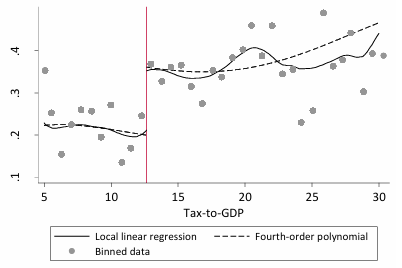
\includegraphics[scale=1.8]{Tax Tipping Point.png}
\caption{Dampak Ambang Pajak terhadap Pertumbuhan PDB Kumulatif 10 Tahun.}
\label{fig:view}
\floatnote{Diagram ini diadaptasi dari \citet{gaspar_2016_tax}, yang menunjukkan hubungan antara rasio pajak terhadap PDB (\textit{tax-to-GDP ratio}) dan pertumbuhan PDB riil kumulatif selama sepuluh tahun pada basis data historis. Titik-titik menggambarkan rata-rata pertumbuhan PDB dalam interval 0,75 poin persentase. Garis penuh merupakan hasil \textit{local linear regression} di kedua sisi ambang 12,65 persen menggunakan \textit{Epanechnikov kernel} dengan \textit{bandwidth} 1,5, sementara garis putus-putus adalah \textit{fourth-order polynomial} dengan pergeseran intersep di titik ambang yang diestimasi.}
\end{figure}

\begin{figure}[hbt!]
\centering
\begin{tikzpicture}[node distance=3cm, thick,  xscale=1.0, yscale=1.2, transform shape]

% Define styles
\tikzstyle{state} = [rectangle, draw, fill=blue!20, text width=3.5cm, text centered, rounded corners, minimum height=1.5em, font=\small]
\tikzstyle{outcome} = [rectangle, draw, fill=green!20, text width=3.5cm, text centered, rounded corners, minimum height=1.5em, font=\small]
\tikzstyle{factor} = [ellipse, draw, fill=yellow!20, text width=2.8cm, text centered, minimum height=1.5em, font=\small]
\tikzstyle{unobs} = [ellipse, draw, fill=gray!20, text width=2cm, text centered, minimum height=1.5em, dashed, font=\small]
\tikzstyle{arrow} = [->, >=latex, thick]
\tikzstyle{doublearrow} = [<->, >=latex, thick]
\tikzstyle{dashedarrow} = [->, >=latex, thick, dashed]

% Layout nodes in a cleaner arrangement
% Top row
\node[factor] (reform) at (-6,6) {Biaya Reformasi};
\node[state] (ins) at (0,6) {Kualitas Institusi};
\node[factor] (trust) at (6,6) {Kepercayaan Publik};

% Middle row
\node[state] (gex) at (-7,3) {Belanja Pemerintah};
\node[unobs] (unobs) at (-3,4) {$U$};
\node[outcome] (peg) at (6,3) {Pertumbuhan Ekonomi};

% Bottom row
\node[factor] (shadow) at (-6,0) {\textit{Shadow Economy}};
\node[state] (tax) at (0,0) {Kapasitas Pajak};
\node[outcome] (revenue) at (6,0) {Penerimaan Negara};

% Main causal relationships dengan path yang lebih jelas
% Bidirectional INS <-> PEG untuk LMICs
\draw[doublearrow] (ins) to[bend right=25] node[midway, right, font=\scriptsize] {LMICs} (peg);

% Direct effects
\draw[arrow] (ins) -- (tax) node[midway, left, font=\scriptsize] {+};
\draw[arrow] (ins) -- (trust) node[midway, above, font=\scriptsize] {+};
\draw[arrow] (trust) -- (tax) node[midway, right, font=\scriptsize] {+};
\draw[arrow] (gex) -- (peg) node[midway, below, font=\scriptsize] {+};
\draw[arrow] (tax) -- (peg) node[midway, below, font=\scriptsize] {+};
\draw[arrow] (tax) -- (revenue) node[midway, below, font=\scriptsize] {+};
\draw[arrow] (shadow) -- (tax) node[midway, below, font=\scriptsize] {-};

% Reform effects
\draw[arrow] (reform) -- (ins) node[midway, above, font=\scriptsize] {+/-};

% Long-run relationship
\draw[arrow, line width=2pt, color=blue!60] (revenue) to[bend right=30] node[midway, below, font=\scriptsize] {Jangka Panjang} (peg);

% Feedback loop
\draw[dashedarrow, color=red!60] (revenue) to[bend left=40] node[midway, left, font=\scriptsize] {feedback} (reform);

% Unobserved confounders dengan path yang jelas
\draw[dashedarrow] (unobs) -- (ins);
\draw[dashedarrow] (unobs) -- (gex);
\draw[dashedarrow] (unobs) to[bend right=15] (tax);

\end{tikzpicture}
\caption{Diagram Kausal: Hubungan Institusi, Kapasitas Pajak, dan Faktor-Faktor Terkait}
\label{fig:integrated_causal}
\floatnote{Diagram ini mengintegrasikan temuan empiris Arvin et al. (2021) dengan faktor-faktor kontekstual tambahan. Variabel disusun dalam tiga tingkat: faktor institusional (atas), proses ekonomi (tengah), dan hasil fiskal (bawah). Garis putus-putus menunjukkan pengaruh variabel tak terobservasi ($U$) dan hubungan feedback.}
\end{figure}

Temuan-temuan ini memperkuat argumen bahwa penguatan tingkat, dalam arti kapasitas pemungutan, pajak bukan sekadar solusi teknis jangka pendek, melainkan bagian dari strategi yang lebih besar—yang pada gilirannya memengaruhi kualitas tata kelola dan kinerja ekonomi secara keseluruhan.

Sebagai penutup bagian ini, penting mengingat perspektif historis yang ditawarkan Brautigam et al. (2008) dalam karya seminalnya tentang \textit{state-building} dan perpajakan di negara berkembang. Ia menegaskan bahwa sistem perpajakan modern di Eropa tidak muncul begitu saja. Ia lahir dari proses negosiasi panjang antara penguasa dan elite ekonomi—di mana pajak ditukar dengan representasi politik dan perlindungan hak properti. 

\begin{quote}
“Taxation is a core governance function. It has the potential to shape relations between state and society in significant and distinctive ways. Tax revenues allow states to provide security and public goods. ‘The history of state revenue production,’ Margaret Levi once wrote, ‘is the history of the evolution of the state.’ For these reasons, taxation should be accorded a central role in analyses of state building.” \citep{brautigam_2008_taxation}
\end{quote}

Indonesia, dengan segala kompleksitas politik dan ekonominya, belum benar-benar melalui proses negosiasi semacam ini hingga tuntas. Mungkin di sinilah letak tantangan kita: bukan hanya soal tarif atau administrasi, tetapi juga tentang membangun kontrak sosial yang membuat pajak dipandang bukan sebagai beban, melainkan sebagai bagian dari kesepakatan bersama dalam membentuk negara yang lebih kuat.

\subsection{Masalah \textit{Transferability}: Vietnam dan Singapura sebagai \textit{False Analogy}?}
Perbandingan dengan Vietnam dan Singapura yang kerap dirujuk Budiawan layak dikaji kembali secara lebih kritis. Vietnam menjalani transisi ekonomi dalam kerangka \textit{political settlement} yang sangat berbeda, dengan dukungan modal asing masif serta konsensus politik yang relatif solid. Reformasi fiskalnya beriringan dengan kebijakan \textit{doi moi} (renovasi ekonomi) yang ditopang bantuan internasional substansial.
\textit{(Konteks ini sulit direplikasi: bukan hanya soal teknis kebijakan, tetapi juga momentum politik yang langka.)}

Singapura, di sisi lain, adalah sebuah \textit{city-state} dengan karakteristik yang hampir tak bisa dibandingkan langsung: perekonomian yang sangat terbuka dan terintegrasi dalam \textit{global value chains}, birokrasi yang ramping dan homogen, serta sistem politik yang memungkinkan perumusan kebijakan jangka panjang tanpa \textit{electoral constraints} yang berarti.
\textit{(Dalam bahasa sederhana: mereka bermain di papan catur yang berbeda, dengan aturan main yang lain pula.)}

\begin{table}[hbt!]
\caption{Indikator Kualitas Institusi: Indonesia vs. Negara Perbandingan (2020)}
\label{tab:institutional_quality}
\centering
\begin{tabular}{lccc}
\textbf{Negara} & \textbf{\textit{Government Effectiveness}} & \textbf{\textit{Corruption Perception}} & \textbf{\textit{Tax-to-GDP Ratio}} \\
\midrule
Singapura & 2,24 & 0,09 & 12,03 \\
Vietnam & -0,31 & 0,69 & 12,8 \\
Thailand & 0,18 & 0,64 & 15,14 \\
Malaysia & 0,43 & 0,52 & 11,64 \\
\textbf{Indonesia} & \textbf{-0,18} & \textbf{0,72} & \textbf{10,4} \\
\end{tabular}
\floatnote{Sumber: World Bank Worldwide Governance Indicators. \textit{Government Effectiveness} berkisar dari -2,5 (terlemah) hingga 2,5 (terkuat). \textit{Corruption Perception} berkisar dari 0 (terbersih) hingga 1 (terkorup).}
\end{table}

Data pada Tabel \ref{tab:institutional_quality} memperlihatkan bahwa Indonesia memang tertinggal dalam indikator kualitas institusi dibanding tetangganya. Namun, kesenjangannya dengan Vietnam tidak terlalu ekstrem. Yang menarik, Vietnam dengan \textit{government effectiveness} yang justru lebih rendah (-0,31 vs -0,18) mampu mencapai \textit{tax ratio} lebih tinggi (12,8 persen vs 10,4 persen).

Hal ini memberi sinyal bahwa faktor-faktor lain—mulai dari struktur ekonomi, \textit{political settlement}, hingga strategi pembangunan—memegang peranan penting.
\textit{(Dengan kata lain, tata kelola memang penting, tetapi ia bukan satu-satunya variabel kunci. Relasi antara kualitas institusi dan \textit{tax ratio} seringkali lebih kompleks, bahkan kontekstual, dibanding yang tersirat dalam kerangka Budiawan.)}

\section{Kesimpulan}
\label{sec:Kesimpulan}
Budiawan patut diapresiasi atas kontribusinya yang signifikan dalam memperkaya wacana publik tentang perpajakan. Peta yang ia susun berangkat dari data yang kuat, observasi yang presisi, dan strategi retorika yang cermat. Ia berhasil mengangkat perdebatan dari sekadar persoalan tarif menuju pembahasan tentang tata kelola dan kapasitas administrasi. Pendekatan ini penting, sebab tanpa fondasi birokrasi yang memadai, kebijakan pajak kerap menjadi wacana tanpa daya paksa. Di tengah debat publik yang sering terjebak pada narasi jangka pendek, intervensi Budiawan mengingatkan kita pada pentingnya stabilitas sistem sebagai syarat awal.

Fokus yang kuat pada optimalisasi administrasi, walau bernilai strategis, menyisakan ruang kosong pada horizon kebijakan. Pajak bukan sekadar masalah teknis yang bisa diselesaikan di ruang rapat kementerian; ia adalah produk dari \textit{political settlement}. Keberhasilan reformasi sering kali ditentukan bukan hanya oleh rapi atau tidaknya sistem administrasi, tetapi oleh kesediaan politik untuk membuka jalur kebijakan baru. Dalam hal ini, Budiawan memilih wilayah yang aman: ia menavigasi peta yang sudah ada tanpa mencoba menandai wilayah tak dikenal yang mungkin berisiko namun potensial.

Pendekatan alternatif mengajak kita melihat pajak sebagai bagian dari proyek politik yang melibatkan negosiasi legitimasi antara negara dan warganya. Kenaikan rasio pajak tidak hanya menuntut perbaikan mekanisme pemungutan, tetapi juga memerlukan kontrak sosial yang meyakinkan publik bahwa beban pajak dibalas dengan manfaat yang nyata. Dalam bahasa sederhana, keberhasilan reformasi fiskal tidak diukur dari berapa persen tarif dinaikkan, tetapi dari sejauh mana publik melihat pajak sebagai investasi bersama.

Peta yang digambarkan Budiawan sudah memuat jalur yang terbukti aman. Tantangan berikutnya adalah membayangkan jalur yang lebih berani: strategi yang mungkin lebih kompleks, bahkan spekulatif, namun memiliki potensi untuk memecah kebuntuan lama. Pendekatan seperti ini bukan berarti meninggalkan prinsip kehati-hatian; ia justru bertolak dari asumsi bahwa stabilitas administrasi adalah landasan bagi inovasi kebijakan. Optimalisasi teknis penting, tetapi imajinasi politik tidak kalah mendesak.

Paradoks fiskal Indonesia tidak akan terselesaikan jika kita hanya bergerak lebih cepat di lintasan yang sama. Ia memerlukan lompatan yang menembus batas lama, disertai peta baru yang menggabungkan ketepatan teknokratis dengan keberanian politik. Budiawan telah memulai langkah penting dengan memperjelas rute yang ada; langkah berikutnya adalah memperluas cakrawala itu. Sejarah reformasi menunjukkan bahwa perubahan besar jarang datang dari jalan utama—ia justru muncul dari jalur sempit yang awalnya tak terlihat, tetapi akhirnya mengubah arah perjalanan.

\clearpage

\nocite{*}
\bibliography{Referensi}

\end{document}
